% 圆锥曲线的极坐标方程

\pentry{极坐标的定义\upref{Polar}}

\subsection{结论}
圆锥曲线的极坐标方程为
\begin{equation}\label{Cone_eq5}
r  = \frac{p}{1 - e\cos \theta }
\end{equation}
其中 $e$ 是离心率, $p$ 是半通径.

\begin{figure}[ht]
\centering
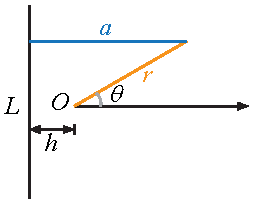
\includegraphics[width=4.5cm]{./figures/Cone1.pdf}
\caption{由离心率定义圆锥曲线}\label{Cone_fig1}
\end{figure}

\subsection{推导}
圆锥曲线的一种定义(与其他定义等效)为(\autoref{Cone_fig1}):
平面上有一点 $O$ 和一条直线 $L$, 相距为 $h$. 
平面上某一点到 $O$ 的距离为 $r$, 到 $L$ 的
(垂直)距离为 $a$, 令常数 $e > 0$, 则所有满足
\begin{equation}\label{Cone_eq1}
r/a = e
\end{equation}
的点组成的曲线就是圆锥曲线. $e$ 是常数,叫做\bb{离心率}, $O$ 是\bb{焦点}, $L$ 是\bb{准线}.当 $0 < e < 1$ 时,曲线是椭圆, $e = 1$ 时是抛物线, $e > 1$ 时是双曲线.

以 $O$ 点为原点,使极轴垂直于准线(如上图).则 $a = h + r \cos \theta $, 根据\autoref{Cone_eq1} 得
\begin{equation}\label{Cone_eq2}
\frac{r}{h + r \cos \theta } = e
\end{equation}
变形,得
\begin{equation}\label{Cone_eq3}
r = \frac{eh}{1 - e\cos \theta }
\end{equation}

\begin{figure}[ht]
\centering
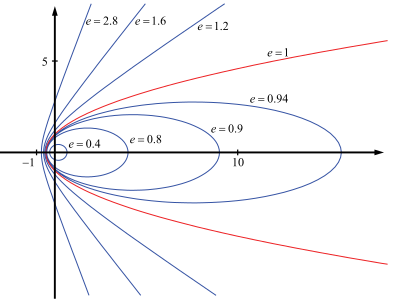
\includegraphics[width=11cm]{./figures/Cone2.pdf}
\caption{不同离心率 $e$ 的圆锥曲线} \label{Cone_fig2}
\end{figure}
若定义圆锥曲线的\bb{通径}为过焦点且平行于准线的直线被圆锥曲线截出的线段,令其长度为 $2p$, 那么有 $r(\pi /2) = p$. 代入\autoref{Cone_eq3} 得 $p = eh$. 所以\autoref{Cone_eq3} 又可以写为
\begin{equation}\label{Cone_eq4}
r  = \frac{p}{1 - e\cos \theta }
\end{equation}


注意 $p$ 和 $e$ 分别控制圆锥曲线的大小和形状.由于抛物线的 $e = 1$ 不变,所以所有抛物线的形状都相同.

\autoref{Cone_eq4} 中一种比较特殊的情况是当圆锥曲线为双曲线($e > 1$)且 $1- e\cos\theta < 0$ 时 $r$ 取负值, 会产生双曲线的左半支(图中未画出). 左半支上的任意一点同样满足\autoref{Cone_eq1}.



